\chapter{How the Internet Works}\index{internet}

You tap a video, and it starts playing in less than a second, even though the server sending it may be
2,000 kilometers away. Meanwhile, your friend across the room is uploading a photo, and someone in
Tokyo is joining a video call. The same wires and radio waves carry all of it, and no single computer is
in charge.

So how does a message find its way from your phone to one particular computer out of billions? This
chapter answers that question in four parts: messages travel as \emph{packets}, every device has an
\emph{IP address}, routers pick paths using the \emph{shortest-path algorithms} you already know, and
\emph{DNS} turns names like \verb|youtube.com| into addresses. In the next chapter, Web APIs, you will
use all of this to send HTTP requests.

\section{A Network of Networks}
The internet is not one network. It is tens of thousands of separate networks that have agreed to pass
each other's messages along. Your home Wi-Fi is a tiny network. It connects to your internet service
provider's network, which connects to bigger networks, which are joined by fiber-optic cables that run
across continents and along the ocean floor.

The devices that join networks together are called \newterm{routers}.\index{router} Your home has one: the
box with the blinking lights. Each router has a simple job. When a message arrives, it looks at where the
message is going and sends it one step closer. No router knows the whole journey.

\section{Packets}\index{packet}
The old telephone network worked by reserving a wire: while you were on a call, a complete circuit from
your phone to your friend's phone belonged to you, even during silences. The internet works differently.
Every message is chopped into small pieces called \newterm{packets}, usually no more than about 1,500
bytes each. Each packet travels on its own, sharing the cables with everyone else's packets.

A packet is like a postcard. Its \newterm{header} is the address side: where it came from, where it is
going, and a sequence number saying which piece of the message it is. Its \newterm{payload} is the
message side.

\textbf{Example}: You send a 3 MB photo (3,000,000 bytes). If each packet carries 1,460 bytes of
payload, how many packets is that?

\textbf{Solution}: $3{,}000{,}000 / 1{,}460 \approx 2{,}054.8$, so it takes 2,055 packets. (The last one is
not full.)

Sharing is what makes the internet efficient, but it has a cost. Packets from the same message can take
different routes, arrive out of order, or get lost when a busy router runs out of room and drops them.

\subsection{TCP: Getting It All, in Order}\index{TCP}
Most of the time, you need every byte: a missing piece of a web page or a photo is a disaster. The
\newterm{Transmission Control Protocol} (TCP) handles this. The receiver uses the sequence numbers to put
the packets back in order and to notice which ones never arrived. It sends back
\newterm{acknowledgments} of what it received, and the sender sends the missing packets again.

Let us simulate it. Create a file called \filename{packets.py}:

\begin{minted}{python}
import random

random.seed(4)
message = "Meet me at the library at 3:30, after band practice."
size = 8   # characters per packet

# Sender: chop the message into numbered packets
packets = []
for start in range(0, len(message), size):
    packets.append((start // size, message[start:start + size]))
print("Sending", len(packets), "packets")

# Receiver: keep the packets that arrive, keyed by number
received = {}
needed = list(range(len(packets)))
round_number = 1

while needed:
    in_flight = [packets[n] for n in needed]
    random.shuffle(in_flight)                  # packets take different routes
    arrived = []
    for number, data in in_flight:
        if random.random() < 0.25:             # 1 packet in 4 gets lost
            continue
        received[number] = data
        arrived.append(number)
    needed = [n for n in range(len(packets)) if n not in received]
    print("Round", round_number, "arrived:", arrived, "still missing:", needed)
    round_number += 1

# Put the packets back in order
print("".join(received[n] for n in range(len(packets))))
\end{minted}

When you run it, you should see:
\begin{verbatim}
Sending 7 packets
Round 1 arrived: [6, 3, 0, 1] still missing: [2, 4, 5]
Round 2 arrived: [2, 5, 4] still missing: []
Meet me at the library at 3:30, after band practice.
\end{verbatim}

The packets arrived scrambled, and three of them were lost, yet the message came out perfectly. (Real
networks lose far fewer than 1 packet in 4; we exaggerated so you can see it happen.)

\subsection{UDP: Fast, No Promises}\index{UDP}
Resending takes time. For a video call or an online game, a packet that arrives half a second late is
worthless: the moment has passed. These programs use the \newterm{User Datagram Protocol} (UDP), which just
sends packets and hopes. If one is lost, the video glitches for an instant and moves on.

\section{IP Addresses}\index{IP address}
Every device on the internet has an \newterm{IP address}, and every packet's header carries the source and
destination addresses. (IP stands for Internet Protocol.) The classic kind, \newterm{IPv4}, is written as
four numbers separated by dots:
$$\texttt{192.168.1.23}$$
Each of the four numbers fits in one byte, so it is between 0 and 255, and the whole address is 32 bits.
That allows $2^{32} = 4{,}294{,}967{,}296$ addresses, about 4.3 billion.

That sounded like plenty in 1981. Today, there are far more phones, laptops, game consoles, and smart
doorbells than that. Two fixes keep things running:
\begin{itemize}
\item \textbf{Private addresses.} Addresses that start with \verb|192.168| or \verb|10| are reserved for use
inside a home or school network. Your home router has one public address on the internet and hands out
private addresses to every device inside. When your laptop sends a packet out, the router swaps in its
public address and remembers where to send the reply. This trick is called \newterm{network address
translation} (NAT).\index{NAT}
\item \textbf{IPv6.}\index{IPv6} The new kind of address is 128 bits long, written in hexadecimal, like
this one:
$$\texttt{2001:db8::8a2e:370:7334}$$
That allows $2^{128} \approx 3.4 \times 10^{38}$ addresses, enough to
never run out.
\end{itemize}

\subsection{Networks Have Prefixes}
Addresses are not handed out at random. A whole network gets a block of addresses that share the same
beginning, called a \newterm{prefix}. The block written \verb|192.168.1.0/24| means ``every address whose
first 24 bits match \verb|192.168.1|''. Since 24 bits is three bytes, that is every address from
\verb|192.168.1.0| to \verb|192.168.1.255|: 256 addresses.

A prefix works like a ZIP code. A mail sorter in Chicago does not need to know every street in Denver; it
only needs to know that everything starting with \verb|802| goes to Denver. In the same way, a router far
away needs only one entry for a whole network, not one for every device in it.

Python's built-in \verb|ipaddress| module understands all of this. Try it in the interpreter:

\begin{minted}{python}
>>> import ipaddress
>>> ip = ipaddress.ip_address("192.168.1.23")
>>> net = ipaddress.ip_network("192.168.1.0/24")
>>> ip in net
True
>>> net.num_addresses
256
>>> int(ip)
3232235799
\end{minted}

The last line shows what the address really is to a computer: one 32-bit number. The dotted form is just
easier for people to read.

\subsection{Ports}\index{port}
An address gets a packet to the right computer, but a computer runs many programs at once. A
\newterm{port} number, also in the header, says which program the packet is for. Web servers listen on
port 443 (or 80 for unencrypted pages). In the Web APIs chapter, your server will listen on port 3000,
which is why you will visit \verb|localhost:3000|. The name \verb|localhost| always means ``this
computer'', at the special address \verb|127.0.0.1|.

\section{Routing: Shortest Paths for Packets}\index{routing}
Now the central question: how does a router decide which way to send a packet?

Picture the routers as the nodes of a graph and the cables between them as the edges. Give each edge a
cost, such as the time in milliseconds a packet takes to cross it. Finding a good route is then exactly
the problem from the Finding Shortest Paths chapter.

\begin{figure}[htbp]
\centering
\begin{tikzpicture}[router/.style={draw, thick, circle, minimum size=0.9cm, fill=blue!8},
                    every edge quotes/.style={fill=white, inner sep=1.5pt, font=\small}]
  \node[router] (A) at (0,1.5) {A};
  \node[router] (B) at (2.5,3) {B};
  \node[router] (C) at (2.5,0) {C};
  \node[router] (D) at (5.5,3) {D};
  \node[router] (E) at (5.5,0) {E};
  \node[router] (F) at (8,1.5) {F};
  \draw[thick] (A) edge["5"] (B) (A) edge["7"] (C) (B) edge["3"] (C) (B) edge["13"] (D)
               (C) edge["4"] (E) (D) edge["6"] (E) (D) edge["2"] (F) (E) edge["15"] (F);
\end{tikzpicture}
\caption{A small network of six routers. Each number is the delay of that link in milliseconds.}
\label{fig:router-network}
\end{figure}

A router does not need the whole path. It only needs to know, for each destination, which neighbor to hand
the packet to: the \newterm{next hop}. The list of next hops is the router's \newterm{forwarding
table}.\index{forwarding table} To build it, the router runs Dijkstra's algorithm from itself, then follows
the \verb|prev| links back from each destination until it reaches the first step.

\textbf{Example}: Find router A's next hop to F.

\textbf{Solution}: Running Dijkstra from A gives these costs: B 5, C 7, E 11 (through C), D 17 (through C
and E), and F 19 (through D). The best path is A $\to$ C $\to$ E $\to$ D $\to$ F. Router A only needs the
first step: send to C. Router C will make its own decision when the packet arrives.

Here is the same computation in Python. Create \filename{routing.py}:

\begin{minted}{python}
import math

# Each router lists its neighbors and the delay (in ms) of each link
links = {
    "A": {"B": 5, "C": 7},
    "B": {"A": 5, "C": 3, "D": 13},
    "C": {"A": 7, "B": 3, "E": 4},
    "D": {"B": 13, "E": 6, "F": 2},
    "E": {"C": 4, "D": 6, "F": 15},
    "F": {"D": 2, "E": 15},
}

def dijkstra(links, origin):
    dist = {router: math.inf for router in links}
    dist[origin] = 0
    prev = {}
    unvisited = set(links)
    while unvisited:
        current = min(unvisited, key=lambda r: dist[r])
        if dist[current] == math.inf:
            break
        unvisited.remove(current)
        for neighbor, delay in links[current].items():
            if dist[current] + delay < dist[neighbor]:
                dist[neighbor] = dist[current] + delay
                prev[neighbor] = current
    return dist, prev

def forwarding_table(links, router):
    dist, prev = dijkstra(links, router)
    table = {}
    for destination in sorted(links):
        if destination == router or destination not in prev:
            continue
        # Walk back from the destination until the step just after the router
        hop = destination
        while prev[hop] != router:
            hop = prev[hop]
        table[destination] = (hop, dist[destination])
    return table

def show(table):
    for destination, (hop, cost) in table.items():
        print(f"  to {destination}: send to {hop}  ({cost} ms)")

print("Router A's forwarding table:")
show(forwarding_table(links, "A"))

# The link between C and E breaks
del links["C"]["E"]
del links["E"]["C"]
print("After the C-E link fails:")
show(forwarding_table(links, "A"))
\end{minted}

The \pyfunction{dijkstra} function is the one from the Finding Shortest Paths chapter, written more
compactly: \verb|min(unvisited, key=...)| finds the unvisited router with the lowest cost in one line.

When you run it, you should see:
\begin{verbatim}
Router A's forwarding table:
  to B: send to B  (5 ms)
  to C: send to C  (7 ms)
  to D: send to C  (17 ms)
  to E: send to C  (11 ms)
  to F: send to C  (19 ms)
After the C-E link fails:
  to B: send to B  (5 ms)
  to C: send to C  (7 ms)
  to D: send to B  (18 ms)
  to E: send to B  (24 ms)
  to F: send to B  (20 ms)
\end{verbatim}

When the C--E cable breaks (perhaps a backhoe digs it up), the routers notice, recompute, and traffic flows
around the damage through B and D. This ability to route around failures is why the internet has no single
point that can bring the whole thing down.

\subsection{Two Ways to Share the Map}
For Dijkstra to work, each router needs the map. Real networks use both of the algorithms from the Finding
Shortest Paths chapter:
\begin{itemize}
\item In \newterm{link-state routing}, every router tells every other router about its own links. Each
router then has the whole map and runs Dijkstra's algorithm itself. The protocol called OSPF works this
way, inside large company and university networks.
\item In \newterm{distance-vector routing}, each router only talks to its neighbors, telling them ``here is
how far I am from every destination.'' Each router updates its own distances from what its neighbors
report, round after round. That is the Bellman-Ford algorithm, spread across many machines. The protocol
called RIP works this way.
\end{itemize}

Between the giant networks that make up the internet, the rules are different. Those networks belong to
competing companies, and their routers (speaking a protocol called BGP) choose paths based on business
agreements as well as speed. The shortest path is not always the one taken.

\subsection{The Speed of Light Is a Speed Limit}\index{latency}
Light in an optical fiber travels at about 200,000 kilometers per second, two-thirds of its speed in a
vacuum. That sets a hard limit on how fast any message can go.

\textbf{Example}: New York and London are about 5,570 km apart. What is the shortest possible time for a
packet to go there and back?

\textbf{Solution}: One way takes $5{,}570 / 200{,}000 = 0.0279$ seconds, about 28 ms. A round trip takes at
least 56 ms. Real cables do not run in perfectly straight lines and routers add delays, so the real time is
more like 70 ms. No amount of engineering can beat 56 ms: that is physics.

This is why online games put servers in many cities, and why video sites keep copies of popular videos close
to you.

\section{DNS: The Internet's Phone Book}\index{DNS}
Nobody wants to type \verb|142.250.72.14| to watch a video. People remember names like \verb|youtube.com|
instead. The \newterm{Domain Name System} (DNS) translates names into IP addresses.

DNS is not one giant list; it is a hierarchy, read from right to left:
\begin{enumerate}
\item Your computer asks a \newterm{resolver}, usually run by your internet provider, for
\verb|www.example.com|.
\item If the resolver does not know, it asks a \newterm{root server}: ``Who handles \verb|.com|?'' There are
13 named root servers, each copied to many places around the world.
\item The root server points to the \verb|.com| servers, which point to the servers for \verb|example.com|.
\item The \verb|example.com| servers give the final answer: the IP address of \verb|www.example.com|.
\end{enumerate}

That is a lot of asking for one web page. To make it fast, every answer comes with a \newterm{time to live}
(TTL), and resolvers \newterm{cache} answers until the TTL runs out. Popular names are almost always already
in the cache, so most lookups take a few milliseconds.

You can look up names yourself. In a terminal, \verb|nslookup example.com| prints the address. In Python:

\begin{minted}{python}
>>> import socket
>>> socket.gethostbyname("localhost")
'127.0.0.1'
>>> socket.gethostbyname("example.com")
\end{minted}

The second lookup needs an internet connection, and the address it prints can change over time, because the
owners of a name can point it at a different server whenever they like. That is one of the best things about
DNS: a website can move to a new computer, and nobody has to learn a new address.

\section{Putting It Together}
Here is what happens when you type \verb|https://www.example.com/| into your browser and press Enter:
\begin{enumerate}
\item \textbf{DNS:} The browser looks up \verb|www.example.com| and gets an IP address.
\item \textbf{TCP:} Your computer and the server exchange three small packets to open a connection, agreeing
on starting sequence numbers.
\item \textbf{Encryption:} Because the address starts with \verb|https|, the two sides agree on a secret key,
using public-key cryptography, the family of ideas behind RSA from the Number Theory and Cryptography chapter. From now
on, routers along the way can see where your packets are going but not what is in them. That is what the
lock icon means.
\item \textbf{HTTP:} The browser sends a request, ``GET this page, please.'' You will learn the details of
HTTP in the Web APIs chapter.
\item \textbf{Routing:} Every packet, in both directions, is passed from router to router, each one choosing
a next hop from its forwarding table.
\item \textbf{Reassembly:} TCP puts the reply's packets back in order, asks again for any that were lost, and
hands the complete page to the browser, which draws it.
\end{enumerate}
All of this usually takes less than a second.

Notice how the jobs are stacked. HTTP does not care how packets are routed, and routers do not care what is
in the packets. Engineers call each job a \newterm{layer}.\index{network layers} Each layer wraps the one
above it, like a letter in an envelope inside a bigger envelope:

\begin{figure}[htbp]
\centering
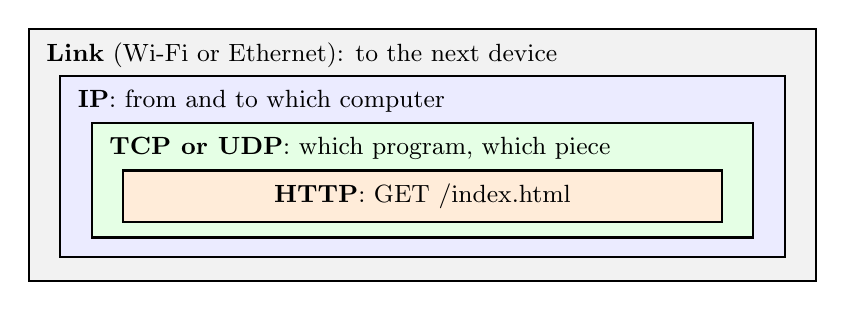
\begin{tikzpicture}[font=\small]
  \draw[thick, fill=gray!10] (0,0) rectangle (10,3.2);
  \node[anchor=north west] at (0.1,3.15) {\textbf{Link} (Wi-Fi or Ethernet): to the next device};
  \draw[thick, fill=blue!8] (0.4,0.3) rectangle (9.6,2.6);
  \node[anchor=north west] at (0.5,2.55) {\textbf{IP}: from and to which computer};
  \draw[thick, fill=green!10] (0.8,0.55) rectangle (9.2,2.0);
  \node[anchor=north west] at (0.9,1.95) {\textbf{TCP or UDP}: which program, which piece};
  \draw[thick, fill=orange!15] (1.2,0.75) rectangle (8.8,1.4);
  \node at (5,1.075) {\textbf{HTTP}: GET /index.html};
\end{tikzpicture}
\caption{The layers of a packet. Each layer adds its own header around the layer inside it.}
\label{fig:layers}
\end{figure}

\begin{Exercise}[title={Counting Packets}, label=in_packets]
A song file is 5 MB (5,000,000 bytes). If each packet carries 1,460 bytes of payload, how many packets does
it take to send it?
\end{Exercise}
\begin{Answer}[ref=in_packets]
$5{,}000{,}000 / 1{,}460 \approx 3{,}424.7$, so it takes 3,425 packets, with the last one only partly full.
\end{Answer}

\begin{Exercise}[title={Video Calls}, label=in_udp]
Why does a video call usually use UDP instead of TCP?
\end{Exercise}
\begin{Answer}[ref=in_udp]
TCP would stop to resend lost packets, and the call would freeze while it waited. By the time a resent
packet arrived, the moment it belongs to would already be over. With UDP, a lost packet causes a tiny
glitch, and the call keeps going in real time.
\end{Answer}

\begin{Exercise}[title={Sizes of Networks}, label=in_prefix]
How many addresses are in the block \verb|10.0.0.0/16|? How many are in a \verb|/8| block?
\end{Exercise}
\begin{Answer}[ref=in_prefix]
An IPv4 address has 32 bits. In a \verb|/16| block, the first 16 bits are fixed and the last 16 are free, so
there are $2^{16} = 65{,}536$ addresses. In a \verb|/8| block, 24 bits are free: $2^{24} = 16{,}777{,}216$
addresses. You can check the first with
\verb|ipaddress.ip_network("10.0.0.0/16").num_addresses|.
\end{Answer}

\begin{Exercise}[title={Enough for Everyone?}, label=in_ipv6]
There are about 8.1 billion people on Earth. If all $2^{128}$ IPv6 addresses were shared equally, how many
would each person get?
\end{Exercise}
\begin{Answer}[ref=in_ipv6]
$2^{128} / (8.1 \times 10^9) \approx 3.4 \times 10^{38} / 8.1 \times 10^9 \approx 4.2 \times 10^{28}$ addresses
per person. IPv4 cannot even give each person one.
\end{Answer}

\begin{Exercise}[title={Router D's Table}, label=in_tableD]
Using the network in Figure~\ref{fig:router-network}, find router D's next hop and cost to each other router.
Check your answer by changing the last lines of \filename{routing.py}.
\end{Exercise}
\begin{Answer}[ref=in_tableD]
From D: F costs 2 (next hop F), E costs 6 (next hop E), C costs 10 (next hop E), B costs 13 (next hop B),
and A costs 17 (next hop E, through E and C). The path to B through E and C also costs 13; the program keeps
the direct link because it found it first. To check, add \verb|show(forwarding_table(links, "D"))| before the
lines that remove the link.
\end{Answer}

\begin{Exercise}[title={Around the World}, label=in_light]
Denver and Tokyo are about 9,330 km apart. What is the shortest possible round-trip time for a packet between
them through optical fiber? Why might an online game feel laggy for a player in Denver on a server in Tokyo?
\end{Exercise}
\begin{Answer}[ref=in_light]
The round trip is $2 \times 9{,}330 = 18{,}660$ km, and $18{,}660 / 200{,}000 \approx 0.093$ seconds, or about
93 ms, before any router delays. In a fast game, a tenth of a second between pressing a button and seeing the
result is easy to feel. Game companies put servers near their players for this reason.
\end{Answer}

\begin{Exercise}[title={Caching Trade-off}, label=in_ttl]
A website sets the TTL of its DNS records to one week. What is good about that? What could go wrong if the
site moves to a new server with a new IP address?
\end{Exercise}
\begin{Answer}[ref=in_ttl]
A long TTL means resolvers rarely need to ask again, so lookups are fast and the site's DNS servers get few
requests. But after the move, resolvers may keep handing out the old, cached address for up to a week, and some
visitors will not find the site. Sites usually shorten the TTL a few days before a planned move.
\end{Answer}

\begin{Exercise}[title={Trace a Route}, label=in_trace]
In a terminal, run \verb|traceroute example.com| (on Windows, \verb|tracert example.com|). Each line is one
router along the way, with the time it took to reply. How many hops does it take? Do you see a place where the
time jumps suddenly? What might cause that?
\end{Exercise}
\begin{Answer}[ref=in_trace]
Answers vary, but most routes take somewhere between 8 and 20 hops. The first hop is your home router. A
sudden jump of tens of milliseconds usually means the packet crossed a long distance, such as across a country
or under an ocean. Some routers do not reply at all and show up as asterisks.
\end{Answer}
